\chapter{Proposta}
Conforme descrito na seção \ref{cap_protocolos_de_roteamento} um protocolo de roteamento é responsável pelo tratamento e pela dinâmica das mensagens e dados trocados entre os dispositivos participantes da comunicação. Como dinâmica pode-se citar o cálculo de rotas a serem utilizadas e, neste sentido, a proposta do presente documento pode ser considerada como um protocolo para estabelecimento de caminhos ótimos de rede através da manipulação do \emph{layer} físico da rede.

O objetivo é a descoberta e estabelecimento de rotas de comunicação de maneira completamente desagregada do protocolo de roteamento utilizado na rede em questão. O protocolo proposto pode ser utilizado em qualquer rede que contenha multi-caminhos ou redundâncias, apesar de apresentar melhores resultados quando aplicado à redes \emph{mesh} devido a maior possibilidade de recombinações. Para tanto, é necessário que a rede em questão possa ser representada por um grafo simples, ou seja, um grafo que não possui arestas paralelas ou pontas coincidentes (laços).

De maneira geral, uma rede \emph{mesh} apresenta vários possíveis caminhos entre o ponto inicial e destino da comunicação, sendo que em cada um desses pontos existem custos atrelados ao roteamento, encaminhamento e processamento de pacotes para qualquer comunicação neste tipo de topologia. A proposta atua no refino destes custos através do estabelecimento de caminhos específicos/estratégicos para cada enlace.

Basicamente existem dois tipos de equipamentos que podem ser utilizados em redes ópticas, os puramente ópticos e os elétricos. Os equipamentos puramente ópticos possuem custo muito elevado e são muito sensíveis, já que têm a capacidade de realizar o roteamento de luz (baseado no comprimento de onda dos sinais) e por isso não são utilizados em larga escala, normalmente esse tipo de tecnologia pode ser encontrado em alguns filtros e \emph{splitters} especiais. Já os equipamentos elétricos possuem custos muito mais atrativos e são normalmente empregados para roteamento de maneira geral, mas em contrapartida são sensivelmente mais lentos.

Os atrasos existentes em equipamentos elétricos utilizados em redes ópticas têm diversas origens, como o processamento dos dados (intrinsecamente relacionado ao poder de processamento do equipamento) e as conversões de meio necessárias, sendo que para cada equipamento pode-se considerar pelo menos duas dessas conversões (óptica-elétrica-óptica). 

Logo, todas as vezes que um pacote trafega em uma rede óptica acaba sofrendo atrasos, que são traduzidos em forma de latência, em cada um dos nós participantes do circuito. Estes atrasos devem ser somados a fim de determinar a latência total de um enlace. A Figura \ref{fig_latency_link} mostra a acúmulo da latência através de um enlace óptico entre dois pontos. 

\begin{figure} [!htb]% normalmente utilizar [!t]
	\centering
	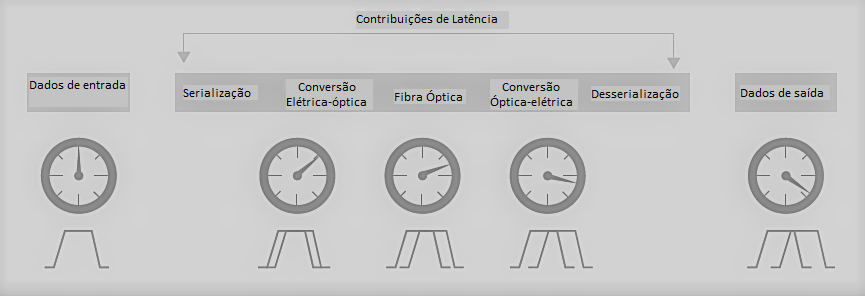
\includegraphics[width=0.5\textwidth]{./figuras/latency-link.png}
	\caption[Latência de Link]{Latência em comunicação entre dois pontos utilizando link óptico. Os principais pontos de inserção de latência na comunicação são resultantes dos processos de conversão elétrica-óptica, transmissão de dados, conversão óptica-elétrica e disponibilização dos dados no destino (desserialização e processamento).}
	\fonte{Adaptado de \cite{Art-Coffe2017}}
	\label{fig_latency_link}
\end{figure}

Logo, a proposta apresentada neste artigo, denominada de \sigla{BSN}{\emph{``Bypass Seletivo de Nós''}} \emph{``Bypass Seletivo de Nós''}, ocupa um lugar intermediário entre os equipamentos puramente ópticos e os ópticos/elétricos. O BSN consiste em um protocolo especificamente desenvolvido para otimização de latência em redes ópticas através da utilização de chaveadores ópticos em pontos estratégicos da rede. Dessa forma equipamentos em posições específicas da rede podem ser desviados sem a necessidade de nenhuma conversão de meio ou mesmo processamento, resultando na mínima inserção de latência possível. 

Os pontos da rede de acionamento do chaveador óptico podem ser escolhidos em ramos de um grafo com muitos vértices (\emph{hops}) ou podem ser planejados para o estabelecimento de rotas específicas para comunicação com pontos críticos do sistema, estabelecendo um \sigla{SLA}{\emph{Service Level Agreement}} em \emph{layer} físico.

Através da utilização do BSN é possível reduzir o grafo da rede possibilitando uma nova configuração de conexões e consequentemente uma nova variedade de rotas possíveis. Cada vez que o BSN ativa um \emph{bypass}, as duas arestas envolvidas são unificadas evitando o vértice das mesmas, criando assim um novo grafo com uma distância entre os dois vértices finais de um vértice a menos, como representado na Figura \ref{fig-bypass-exemplo}. Dessa forma, em caso de falha ou mudança de SLA, a topologia física pode ser alterada automaticamente.

\begin{figure} % normalmente utilizar [!t]
	\centering
	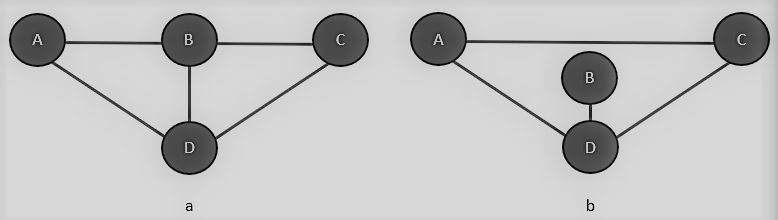
\includegraphics[width=0.5\textwidth]{./figuras/Bypass-exemplo-PB.png}
	\caption[Exemplo de atuação de \emph{by-pass} óptico]{Efeito da utilização do chaveador ótico. Em ``a'' pode-se ver a rede original contendo dois saltos entre os vértices A e C. Em ``b'' após o acionamento do dispositivo no vértice B pode-se ver e existência de apenas um salto entre os vértices A e C}
	\label{fig-bypass-exemplo}
\end{figure}

\section{Computação Evolucional e Inteligência Artificial}
Comumente conhecida como \sigla{IA}{Inteligência Artificial} (Inteligência Artificial) ou \sigla{AI}{\emph{Artificial Intelligence}} (\emph{Artificial Intelligence}, a Inteligência Artificial pode ser considerada como um campo de pesquisa multidisciplinar ligado ao desenvolvimento e investigação de sistemas inteligentes \cite{Book-Brownlee2011}. Segundo \cite{Book-Russel2009} a IA pode ser dividida em 4 categorias: sistemas que pensam como humanos, sistemas que agem como humanos, sistemas que pensam com razão e sistemas que agem com razão.

Um dos campos comumente relacionados à IA é a Computação Evolucionária ou \sigla{CE}{Computação Evolucionária}, que foi inicialmente concebida por Lawrence J. Fogel em meados de 1960 e pode ser representada como a junção de diferentes abordagens de simulação de aspectos da evolução. Todas estas abordagens envolvem aspectos em comum como reprodução, aleatoriedade ou mutação, competição e seleção. Até o surgimento da CE a IA estava, em sua maioria, focada em heurísticas e simulações de redes neurais primitivas. Abordagens estas que mostravam-se, segundo Fogel, limitadas já que produzem modelos muito mais próximos de um comportamento humano do que de um processo envolvido na criação de indivíduos ou intelectos (evolução) \cite{Book-Back2000}.

De maneira geral a evolução é um processo de otimização, o que definitivamente não implica em perfeição, aliado à grande robustez de adaptação visto que o mundo real nunca é estático \cite{Book-Back2000}.

Uma das classes dos algoritmos evolucionários mais difundidas e utilizadas são os Algoritmos Genéticos ou \sigla{AG}{Algoritmos Genéticos}. Estes algoritmos são caracterizados por serem uma técnica de otimização global através de estratégias adaptativas. Eles são assim chamados por serem inspirados na genética e evolução de populações e por isso se utilizam de nomenclaturas como \emph{cromossomos, genes, recombinação, mutação, etc} \cite{Book-Brownlee2011}.

De maneira básica e generalista pode-se dizer que uma população inicial de indivíduos devidamente correlacionados com o problema em questão é gerada, normalmente de maneira aleatória, e cada indivíduo é avaliado separadamente estabelecendo um \emph{ranking} (normalmente chamado de \emph{fitness}) dos mais adaptados ao problema sob análise. Então, alguns indivíduos da população são selecionados para reprodução, sendo que os indivíduos mais adaptados usualmente recebem mais chances de participar deste processo. Além disso, também existe a mutação que visa alterar o conteúdo genético de um indivíduo aleatoriamente, diferenciando-o de seus pais. Para o surgimento da nova geração os indivíduos gerados (filhos) devem ser unidos aos seus pais e deve existir um método de seleção de indivíduos a fim de evitar o aumento descontrolado da população \cite{Book-Back2000}. Existem diversas técnicas diferentes para cada um dos passos acima descritos, cada uma delas deve influenciar o algoritmo de maneira diferente (tempo de execução, utilização de memória, processamento utilizado, etc) mas apesar de não existirem garantias, em qualquer um dos casos espera-se encontrar o valor ótimo para a função avaliada. O Algoritmo \ref{pseudocode_AG} é uma representação em alto nível da estratégia básica de um AG. 

\begin{algorithm} [h]
\caption{ - Exemplo de alto nível para AG}
\begin{algorithmic}[1]
\State $Population\gets \textit{InitializePopulation}$
\State EvaluatePopulation(Population);
\State $Sbest\gets \textit{GetBestSolution(Population)}$
\While {$ StopCondition() $}
\State $Parents\gets \textit{SelectParents(Population,PopulationSize)}$
\State $Children\gets 0$
\ForEach {$Parent1, Parent2 \in Parents $}
\State $Child1, Child2 \gets Crossover(Parent1, Parent2)$
\State $Children \gets Mutate(Child1)$
\State $Children \gets Mutate(Child2)$
\EndFor
\State EvaluatePopulation(Children);
\State $Sbest\gets \textit{GetBestSolution(Children)}$
\State $Population\gets \textit{Replace(Population,Children)}$
\EndWhile
\State\Return Sbest
\end{algorithmic}
\fonte{Adaptado de \cite{Book-Brownlee2011}}
\label{pseudocode_AG}
\end{algorithm}


%Inserir descrição sobre Inteligencia artificial e algoritmos genéticos

\section{BSN}
O método de redução do grafo de rede utilizado pelo BSN é descrito sucintamente em alto nível através do pseudocódigo representado no Algoritmo \ref{pseudocode_bsn}. O BSN utiliza vários conceitos de otimização simultâneos. A ideia básica é a utilização de um algoritmo genético para a criação de diferentes combinações de estado dos chaveadores óticos na rede (de acordo com as premissas de projeto a serem adotadas). Dessa forma, cada uma das combinações geradas pelo algoritmo genético acaba por gerar uma nova topologia de conexões físicas, que são por sua vez otimizadas buscando obter a rede menos profunda possível. Para o passo representado na linha \ref{bsn:fitness_line} do Algoritmo \ref{pseudocode_bsn} (busca local), pode ser utilizado qualquer algoritmo conhecido sendo que o presente documento utilizou uma busca de custo uniforme, garantindo assim a obtenção do valor ótimo de \emph{fitness}.

\begin{algorithm} [h]
\caption{ - Algoritmo básico do BSN}
\begin{algorithmic}[1]
\State $popsize\gets \textit{tamanho da populacao}$
\State $gennumb\gets \textit{numero de geracoes}$\\
\State PopList[] = new List[popsize]\Comment{Variável para alocação da geração atual}
\State $i\gets 0$
\While {$ i< popsize $}
\State Individuo = CriaIndividuo()\Comment{Cria a uma configuração de rede}
\State CalculaFit(Individuo)\label{bsn:fitness_line}\Comment{Realiza busca local na instância de rede}
\State PopList.Add(Individuo)\Comment{Adiciona a instância de rede à lista}
\State PopList.ClassifcaIndividuos()\Comment{Organiza a população atual de acordo com o Fitness individual}
\EndWhile\Comment{População inicial criada}\\
\State $j\gets 1$
\While {$ j< gennumb $}\Comment{Roda algoritmo genético}
\State ParentsList[] = new List[]\Comment{Variável para alocação de indivíduos ``pais''}
\State NewList[] = new List[popsize]\Comment{Variável para alocação de próxima geração}
\State ParentsList = SelecionaIndividuos(PopList)\Comment{Seleciona os indivíduos da geração atual que serão utilizados para criação da geração seguinte}
\State NewList = CrossOver(ParentsList)\Comment{Cruza os indivíduos selecionados}
\State Mutation(NewList)\Comment{Aplica algoritmo de mutação de genes na nova população}
\State PopList = MesclaGen(NewList, PopList)\Comment{Realiza elitismo de indivíduos}
\State PopList.ClassifcaIndividuos()\Comment{Organiza a população atual de acordo com o Fitness individual}
\EndWhile\\
\State\Return PopList.Individuo(0)\Comment{Retorna melhor instância de rede}
\end{algorithmic}
\label{pseudocode_bsn}
\end{algorithm}

